% -*- coding: utf-8; -*-

%% https://linorg.usp.br/CTAN/macros/latex/required/tools/longtable.pdf %%
%% http://ctan.dcc.uchile.cl/macros/latex/required/tools/longtable.pdf %%

\chapter{Casos de Uso}
\label{cha:Casos de Uso}

Os casos de uso do sistema servem para descrever como o sistema pode ser utilizado afim de se satisfazer as necessidades do usuário.
Os casos de uso referenciam os requisitos do sistema descritos no capítulo \ref{cha:Requisitos}.
A figura \ref{fig:diagrama-casos-uso} contém o diagrama de casos de uso do sistema.

\begin{figure}[ht]
    \begin{center}
    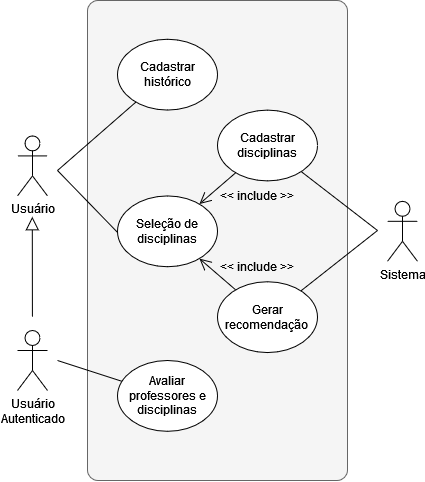
\includegraphics[width=250pt]{figuras/casos-uso.png}
    \caption{Diagrama dos casos de uso}
    \label{fig:diagrama-casos-uso}
    \end{center}
\end{figure}

A seguir estão as descrições dos casos de uso presentes na figura \ref{fig:diagrama-casos-uso}.

\begin{longtable}{ | m{0.3\textwidth} | m{0.7\textwidth} | }
    \hline\hline
    \multicolumn{2}{|c|}{Caso de Uso \textbf{UC01} - Cadastrar disciplinas}\tabularnewline\hline\hline\endfirsthead
    \hline\hline
    \multicolumn{2}{|c|}{Caso de Uso \textbf{UC01} (continuação)}\tabularnewline\hline\hline\endhead
    \hline\endfoot
    \hline\caption{Caso de uso UC01}\endlastfoot

    \textbf{Objetivo} & Permitir que o sistema atualize as disciplinas e suas informações no banco de dados, incluindo as eletivas.\tabularnewline\hline 
    \textbf{Requisitos} & RF01, RF09, RF18 e RF19\tabularnewline\hline
    \textbf{Atores} & Sistema\tabularnewline\hline
    \textbf{Pré condições} & Não se aplica\tabularnewline\hline

    \multirow{1}{*}{\textbf{Fluxo principal}} & [1] O sistema acessa o microhorário, coletando informações de todas as disciplinas.\tabularnewline\cline{2-2}
    & [2] O sistema trata e converte as informações para o modelo do banco.\tabularnewline\cline{2-2}
    & [3] O sistema armazena as novas informações no banco.\tabularnewline\cline{2-2}
    & [4] O sistema atualiza a data e hora da última atualização do microhorário que aparece na interface.\tabularnewline\cline{2-2}
    & [5] O caso de uso é encerrado.
    \label{tab:uc01}
\end{longtable}


\begin{longtable}{ | m{0.3\textwidth} | m{0.7\textwidth} | }
    
    \hline\hline    
    \multicolumn{2}{|c|}{Caso de Uso \textbf{UC02} - Cadastrar histórico}\tabularnewline\hline\hline\endfirsthead
    \hline\hline
    \multicolumn{2}{|c|}{Caso de Uso \textbf{UC02} (continuação)}\tabularnewline\hline\hline\endhead
    \hline\endfoot
    \hline\caption{Caso de uso UC02}\endlastfoot

    \textbf{Objetivo} & Permitir que o usuário cadastre seu histórico escolar no sistema para personalizar as recomendações.\tabularnewline\hline
    \textbf{Requisitos} & RF02, RF04, RF08\tabularnewline\hline
    \textbf{Atores} & Usuário\tabularnewline\hline
    \textbf{Pré condições} & O usuário seleciona a opção de cadastrar histórico.\tabularnewline\hline

    \multirow{1}{*}{\textbf{Fluxo principal}} & [1] O sistema exibe uma tela sobreposta solicitando o histórico escolar do aluno.\tabularnewline\cline{2-2}
    & [2] O usuário submete o histórico escolar. \textbf{[A1]}\tabularnewline\cline{2-2}
    & [3] O sistema armazena o histórico e o currículo do aluno.\tabularnewline\cline{2-2}
    & [4] O sistema exibe um texto de histórico cadastrado com sucesso. \textbf{[A2]}\tabularnewline\cline{2-2}
    & [5] O caso de uso é encerrado.\tabularnewline\hline

    \multirow{1}{*}{\textbf{Fluxos Alternativos}} & \textbf{[A1] O usuário pressiona fora da tela de cadastro de histórico}\tabularnewline\cline{2-2}
    & [1] O caso de uso é encerrado.\tabularnewline\cline{2-2}

    & \textbf{[A2] O sistema não consegue encontrar o currículo ou as disciplinas cursadas no currículo}\tabularnewline\cline{2-2}
    & [1] O sistema exibe um texto de erro.\tabularnewline\cline{2-2}
    & [2] O sistema volta para o passo 1 do fluxo principal. 
    \label{tab:uc02}
\end{longtable}


\begin{longtable}{ | m{0.3\textwidth} | m{0.7\textwidth} | }
    \hline\hline
    \multicolumn{2}{|c|}{Caso de Uso \textbf{UC03} - Gerar recomendações}\tabularnewline\hline\hline\endfirsthead
    \hline\hline
    \multicolumn{2}{|c|}{Caso de Uso \textbf{UC03} (continuação)}\tabularnewline\hline\hline\endhead
    \hline\endfoot
    \hline\caption{Caso de uso UC03}\endlastfoot

    \textbf{Objetivo} & Permitir que o sistema recomende disciplinas para o usuário.\tabularnewline\hline 
    \textbf{Requisitos} & RF01-06, RNF01-02\tabularnewline\hline
    \textbf{Atores} & Sistema\tabularnewline\hline
    \textbf{Pré condições} & O usuário modificou a grade horária.\tabularnewline\hline

    \multirow{1}{*}{\textbf{Fluxo principal}} & [1] O sistema coleta as disciplinas e turmas já adicionadas no grade horária do usuário.\tabularnewline\cline{2-2}
    & [2] O sistema recupera o histórico escolar do usuário do banco de dados, caso o usuário esteja autenticado e o tenha submetido.\textbf{[A1]}\tabularnewline\cline{2-2}
    & [3] O sistema utiliza o algoritmo para gerar recomendações de disciplinas para o usuário.\tabularnewline\cline{2-2}
    & [4] O sistema exibe as recomendações na interface do usuário\tabularnewline\cline{2-2}
    & [5] O caso de uso é encerrado.
    \label{tab:uc03}
\end{longtable}


\begin{longtable}{ | m{0.3\textwidth} | m{0.7\textwidth} | }
    
    \hline\hline
    \multicolumn{2}{|c|}{Caso de Uso \textbf{UC04} - Selecionar disciplina}\tabularnewline\hline\hline\endfirsthead
    \hline\hline
    \multicolumn{2}{|c|}{Caso de Uso \textbf{UC04} (continuação)}\tabularnewline\hline\hline\endhead
    \hline\endfoot
    \hline\caption{Caso de uso UC04}\endlastfoot

    \textbf{Objetivo} & Permitir que o usuário adicione e remova disciplinas da sua grade.\tabularnewline\hline
    \textbf{Requisitos} & RF1\tabularnewline\hline
    \textbf{Atores} & Usuário\tabularnewline\hline
    \textbf{Pré condições} & O usuário está na área de criação da grade horária.\tabularnewline\hline

    \multirow{1}{*}{\textbf{Fluxo principal}} & [1] O sistema exibe a grade horária do usuário, uma lista de disciplinas disponíveis, uma lista de disciplinas recomendadas e um campo de texto para pesquisa.\tabularnewline\cline{2-2}
    & [2] O usuário seleciona uma disciplina da lista de disciplinas disponíveis ou recomendadas. \textbf{[A1]} \textbf{[A2]} .\tabularnewline\cline{2-2}
    & [3] O sistema exibe as turmas disponíveis para a disciplina selecionada e um botão de voltar.\tabularnewline\cline{2-2}
    & [4] O usuário seleciona uma das turmas exibidas. \textbf{[A3]}\tabularnewline\cline{2-2}
    & [5] O sistema acrescenta a turma selecionada na grade horária, e recalcula as disciplinas recomendadas. \tabularnewline\cline{2-2}
    & [6] O caso de uso é encerrado.\tabularnewline\hline

    \multirow{1}{*}{\textbf{Fluxos Alternativos}} & \textbf{[A1] O sistema seleciona uma das disciplinas na sua grade horária}\tabularnewline\cline{2-2}
    & [1] O sistema exibe um botão de informação e um botão de excluir.\tabularnewline\cline{2-2} 
    & [2] O usuário seleciona o botão de excluir.\textbf{[A3]}\tabularnewline\cline{2-2} 
    & [3] O sistema remove a turma e disciplina da grade horária do usuário, e recalcula as disciplinas recomendadas. \tabularnewline\cline{2-2}
    & [4] O sistema volta para o passo 1 do fluxo principal. \tabularnewline\cline{2-2}

    & \textbf{[A2] O usuário preenche o campo de texto para pesquisa}\tabularnewline\cline{2-2}
    & [1] O sistema altera a lista de disciplinas, filtrando de acordo com o texto do campo de pesquisa. \tabularnewline\cline{2-2}
    & [2] O sistema volta para o passo 1 do fluxo principal. \tabularnewline\cline{2-2}

    & \textbf{[A3] O usuário pressiona o botão de informação}\tabularnewline\cline{2-2}
    & [1] O sistema volta para o passo 3 do fluxo principal. %% \tabularnewline\cline{2-2}

    \label{tab:uc04}
\end{longtable}


\begin{longtable}{ | m{0.3\textwidth} | m{0.7\textwidth} | }
    \hline\hline
    \multicolumn{2}{|c|}{Caso de Uso \textbf{UC05} - Avaliar disciplinas e professores}\tabularnewline\hline\hline\endfirsthead
    \hline\hline
    \multicolumn{2}{|c|}{Caso de Uso \textbf{UC05} (continuação)}\tabularnewline\hline\hline\endhead
    \hline\endfoot
    \hline\caption{Caso de uso UC05}\endlastfoot

    \textbf{Objetivo} & Permitir que o usuário avalie uma disciplina ou um professor.\tabularnewline\hline
    \textbf{Requisitos} & RF03, RF15 e RF16\tabularnewline\hline
    \textbf{Atores} & Usuário\tabularnewline\hline
    \textbf{Pré condições} & Não se aplica.\tabularnewline\hline

    \multirow{1}{*}{\textbf{Fluxo principal}} & [1] O sistema exibe uma lista de disciplinas e professores e um campo de texto para pesquisa.\tabularnewline\cline{2-2}
    & [2] O usuário seleciona uma disciplina. \textbf{[A1]} \textbf{[A2]}\tabularnewline\cline{2-2}
    & [3] O sistema exibe uma tela para avaliar a disciplina, um botão de salvar e um botão de voltar.\tabularnewline\cline{2-2}
    & [4] O usuário avalia a disciplina e seleciona o botão de salvar. \textbf{[A3]}\tabularnewline\cline{2-2}
    & [5] O sistema armazena a avaliação do usuário.\tabularnewline\cline{2-2}
    & [6] O caso de uso é encerrado.\tabularnewline\hline

    \multirow{1}{*}{\textbf{Fluxos Alternativos}} & \textbf{[A1] O usuário seleciona um professor}\tabularnewline\cline{2-2}
    & [1] O sistema exibe uma tela para avaliar o professor, um botão de salvar e um botão de voltar.\tabularnewline\cline{2-2}
    & [2] O usuário avalia o professor e seleciona o botão de salvar. \textbf{[A3]}\tabularnewline\cline{2-2} 
    & [3] O sistema armazena a avaliação do usuário.\tabularnewline\cline{2-2}
    & [4] O caso de uso é encerrado.\tabularnewline\cline{2-2}

    & \textbf{[A2] O usuário preenche o campo de texto para pesquisa}\tabularnewline\cline{2-2}
    & [1] O sistema exibe disciplinas e professores utilizando como filtro o texto do usuário.\tabularnewline\cline{2-2}
    & [2] O sistema volta para o passo 1 do fluxo principal.\tabularnewline\cline{2-2}

    & \textbf{[A2] O usuário seleciona o botão de voltar}\tabularnewline\cline{2-2}
    & [2] O sistema volta para o passo 1 do fluxo principal. %%\tabularnewline\cline{2-2} 

    \label{tab:uc05}
\end{longtable}
